\chapter[Introduction to the Template: Motivation and First Steps]{Introduction to the Template Motivation and First Steps}
\label{cp:introduction}

{
	\parindent0pt

	\textit{Author: Gaurav Raj}

	\textit{License: \LaTeX~GPLv3}

	\textit{Official Repository: \href{https://github.com/thehackersbrain/thesis-template}{GitHub Repository}}

	\vspace{.935em}

	Welcome to the \textcolor{maincolor}{\textit{Thesis Template}} template! Thank you for choosing it for your dissertation, report, or project. This template reflects many hours of development, and I hope you enjoy using it as much as I did creating it. This chapter introduces its purpose and helps you get started. See \autoref{cp:user-guide} for a detailed guide, and \autoref{cp:latex-tutorial} for a brief \LaTeX~tutorial to maximise its use.
}

\section{Motivation}
I've been using \LaTeX~since 2020 for a wide range of purposes. Over time, I've reviewed over a hundred templates, and there's always something missing. \textit{Always}. Powerful templates---\textit{i.e.}, highly customisable with many options---are often poorly organised. Well-organised ones usually lack flexibility. Some even compile with errors and warnings. Most importantly, many aren't user-friendly. So, I created my own template for theses and reports, tailored to the Polytechnic University of Leiria. My goals were: \(i)\) clear and structured file organisation, \(ii)\) a clean, professional, and attractive design, \(iii)\) high customisability, and \(iv)\) ease of use, especially for beginners.


\section{Getting Started}
To start using this template, you first need to know how to use \LaTeX. For this, please refer to \autoref{cp:latex-tutorial}. Once you are familiar with \LaTeX, you will need to either install it locally or use an online \LaTeX~editor.

If you prefer an online editor, I highly recommend \href{https://www.overleaf.com/}{Overleaf}. While Overleaf offers a paid subscription for extended compilation time, this template is specifically designed to compile within the limits of the free subscription plan. To use the template in Overleaf, just refer to \href{https://www.overleaf.com/latex/templates/unofficial-polytechnic-university-of-leiria-estg-thesis-slash-report-template/tqgbrncfhwgt}{official template page} and click \textit{Use as Template}. But if you prefer to use a different version of it (which I do not recommend), you can do the following:

\begin{enumerate}[font=\itshape]
	\setlength{\itemsep}{.375em}
	\item \textit{Download the \href{https://github.com/joseareia/ipleiria-thesis/releases}{desired version} from the GitHub repository as a Zip file.}
	\item \textit{Login to your Overleaf account.}
	\item \textit{In your Project area, click in the menu and then: New Project \(\to\) Upload Project.}
	\item \textit{Upload the Zip file.}
	\item \textit{Let Overleaf compile the document.}
\end{enumerate}

If you choose to use a local editor, you must first install \LaTeX~on your machine. For this, there are several options, but I personally recommend either \href{https://www.tug.org/texlive/}{TeX-Live} or \href{https://miktex.org/}{MikTeX}. After installing \LaTeX, you will need to select an editor for writing and editing your documents. To help with this decision, I suggest checking out this helpful \href{https://tex.stackexchange.com/questions/339/latex-editors-ides}{post}, which provides a comprehensive overview of various editors you can use. Once \LaTeX~and your editor are set up, simply clone or download the \href{https://github.com/joseareia/ipleiria-thesis/releases}{latest} version of the template from GitHub and start using it!

\begin{block}[tip]
	In the official GitHub repository, you'll find a \href{https://github.com/joseareia/ipleiria-thesis/blob/master/Makefile}{Makefile} and a \href{https://github.com/joseareia/ipleiria-thesis/blob/master/.latexmkrc}{Latexmk configuration file}, either of which can be used to compile the project. The Makefile supports both \texttt{rubber} and \texttt{latexmk} as compilers, so you can choose the one that best suits your preferences.
\end{block}

\section{Getting Help}
As a newcomer, you may encounter situations where you want to do something in \LaTeX~or with this template but aren't sure how. When questions arise, you have several options. First, you can read the wiki available in the \href{https://github.com/joseareia/ipleiria-thesis}{GitHub} repository for this template. Another great option is the \href{https://tex.stackexchange.com/}{TeX Stack Exchange}, an active community that can help with nearly any issue. Of course, Google is always a reliable resource. If all else fails, feel free to contact me directly with any questions about the template. You can reach me at \textit{\textcolor{blue}{\ul{jose.apareia@gmail.com}}}.

\subsection{Issues, Feature Request and Suggestions}
If, by any chance, you encounter a bug, have a suggestion, or would like to request a feature, you can submit them via the \textit{Issues} tab in the \href{https://github.com/joseareia/ipleiria-thesis}{GitHub} repository. Please be as descriptive as possible when reporting issues, and make sure to provide the appropriate labels to help me triage them effectively.

For feature requests or suggestions, you can either follow the steps mentioned above or, if you prefer, you can implement the feature yourself and submit a pull request. Both pull requests and pushes trigger a \href{https://github.com/joseareia/ipleiria-thesis/actions/workflows/latex.yml}{GitHub Action} that will automatically compile the document. If the compilation fails, the pull request will be automatically rejected. Please keep this in mind and take care when submitting changes.

\subsection{In-Built Comments, Guidance Texts and Warnings}
Within this document template, you may encounter informational text displaying the message ``Writing Guidance.'' These sections are provided solely as guidance to help users understand what content should be included in specific sections. They are not related to the \LaTeX~code itself within this template.

While navigating through the template, especially the configuration files, you will notice that everything is thoroughly commented. \LaTeX~can sometimes be difficult to understand without proper documentation for the packages we are working with. With that in mind, I have made an effort to comment on all the changes I’ve made. Occasionally, I may forget or deem it unnecessary to comment on simpler changes, but more advanced modifications are always accompanied by detailed comments.

Finally, regarding warnings: please take them into consideration when compiling the document. As you may have noticed, the template is designed to be free of warnings, so please strive to maintain this clean compilation.

\section{Important Notices}
Although this template is specifically tailored for students from all six schools of the Polytechnic University of Leiria, you are welcome to use it if you are from a different institution. It is highly customisable and can be easily modified to suit the needs of other schools. If your school is interested in adopting this as the official template, please contact me first.

If you decide to use this template, please consider acknowledging it in your work. To do so, simply cite it using \verb|\citep{IPLeiriaThesis}|. You can also show your appreciation for this template by giving a \href{https://github.com/joseareia/ipleiria-thesis/stargazers}{star} on the GitHub repository. This helps increase its visibility, and you will receive notifications about the latest updates and releases. Either way, acknowledging this work, which involved significant effort and countless hours, would be greatly appreciated.

\section{Another Important Note}
Okay, My emacs setup is finally working and is awesome.

\section{Maths Testing}
This is the section to plot maths graphs.

\vspace{10pt}

\begin{figure}[h]
	\begin{center}
		\begin{tikzpicture}
			\begin{axis}[
					axis lines=middle,
					xlabel={$t$},
					ylabel={$v$},
					xmin=-0.2, xmax=1,
					ymin=-40, ymax=70,
					xtick={0},
					ytick={-30,0,60},
					width=10cm,
					height=8cm,
					axis line style={->},
					ticklabel style={font=\small}
				]

				\addplot[domain=0:0.5, thick]{60};
				\addplot[domain=0:0.5, thick, dashed]{-30};

				\draw[dashed] (axis cs:0.5,0) -- (axis cs:0.5,-30);
				\draw[dashed] (axis cs:0.5,60) -- (axis cs:0.5,0);

				\node at (axis cs:0.5,62) [anchor=west] {$v = \SI{60}{\metre\per\second}$};
				\node at (axis cs:0.5,-30) [anchor=west] {$v = -30$};
				\node at (axis cs:0.25,30) {Area 30};
				\node at (axis cs:0.25,-15) {Area -15};
				\node at (axis cs:0.5,0) [below, xshift=6pt] {$\tfrac{1}{2}$};

			\end{axis}
		\end{tikzpicture}
	\end{center}
\end{figure}
\vspace{10pt}

\subsection{Formulas}

Now Formulas, a basic \textbf{Quadratic Equation} cheatcode formula

\[
	x = \frac{-b \pm \sqrt{b^{2} - 4ac}}{2a}
\]

\vspace{10pt}

Now let's get a bit advanced.

\vspace{20pt}

\newpage

\subsection{Function Plots}

You think trigonometry is only for navigaters. Think again. Some of the best use cases of trigonometry is in \textbf{\textit{rotation}}, \textbf{\textit{vibration}}, and \textbf{\textit{Oscillation}}. Basically in repeating patterns or motions.

\vspace{\baselineskip}

Here's a simple \textbf{\textit{Sinusoidal Oscillation}}.

\vspace{10pt}

\begin{figure}[h]
	\centering
	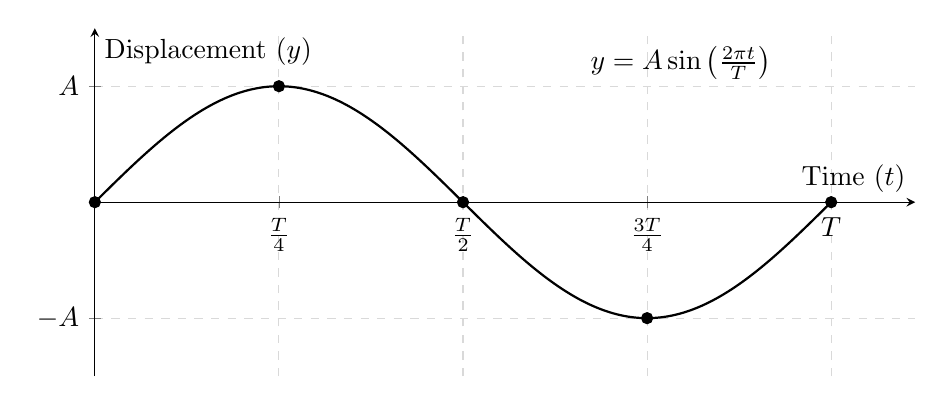
\begin{tikzpicture}
		\begin{axis}[
				width=12cm,
				height=6cm,
				axis lines=center,
				xlabel={Time $(t)$},
				ylabel={Displacement $(y)$},
				xmin=0, xmax=7,
				ymin=-1.5, ymax=1.5,
				xtick={0, 1.5708, 3.14159, 4.7124, 6.2832},
				xticklabels={0, $\frac{T}{4}$, $\frac{T}{2}$, $\frac{3T}{4}$, $T$},
				ytick={-1, 0, 1},
				yticklabels={$-A$, 0, $A$},
				samples=200,
				domain=0:6.2832,
				grid=major,
				grid style={dashed, gray!30},
			]

			% Plot sine wave
			\addplot[thick, black] {sin(deg(x))};

			% Mark key points
			\addplot[mark=*, mark size=2pt, black] coordinates {(0, 0)};
			\addplot[mark=*, mark size=2pt, black] coordinates {(1.5708, 1)};
			\addplot[mark=*, mark size=2pt, black] coordinates {(3.14159, 0)};
			\addplot[mark=*, mark size=2pt, black] coordinates {(4.7124, -1)};
			\addplot[mark=*, mark size=2pt, black] coordinates {(6.2832, 0)};

			% Function label
			\node at (axis cs:5, 1.2) {$y = A\sin\left(\frac{2\pi t}{T}\right)$};

		\end{axis}
	\end{tikzpicture}

	\caption{Sinusoidal oscillation showing one complete period $T$ with amplitude $A$.}
	\label{fig:sine_oscillation}
\end{figure}

\vspace{20pt}

\subsection{Theorems}

\begin{theorem}
	For all $a,b \in \mathbb{R}$, $(a+b)^2 = a^2 + 2ab + b^2$.
\end{theorem}
